\documentclass[a4paper,10pt]{article}
\usepackage[utf8]{inputenc}
\usepackage{amsmath}
\usepackage{amsfonts}
\usepackage{amssymb}
\usepackage{graphicx}
\usepackage{tikz}
\usepackage{amsthm}
%opening
\title{Parallel computation of the sequence of iterates of a function }
\author{Jean-Michel Fourneau \and Maël Guiraud \and Yann Strozecki}
\newcommand{\cS}{\mathcal{S}}
\newcommand{\todo}[1]{{\color{red} TODO: {#1}}}

 \newtheorem{theorem}{Theorem}
 
\begin{document}

\maketitle

\begin{abstract}

\end{abstract}

\section{Model}

Let $\cS$ be a finite set of states and let $f$ be a computable function from $\cS$ to $\cS$. 
The aim of this short article is to propose practical methods to compute the sequence $(s,f(s),\dots,f^n(s))$ in parallel.
When it is possible to compute efficiently $f^i(s)$ using only $s$ and $i$, it is easy to compute the sequence
in parallel by assigning one $f^i(s)$ to each processor. However, for general $f$ we need $f^{i}(s)$ to compute $f^{i+1}(s)$ and there is no simple scheme to parallelize the computation of the sequence. 
Hence, we consider additional structure on $\cS$ to make the problem tractable. The set $\cS$ is equipped with a partial order 
$\leq$ and it has a smallest element $\bot$ and a greatest element $ \top$. We assume that $f$ is monotone, that is 
if $s_1$ and $s_2$ are elements of $\cS$ such that $s_1 \leq s_2$ then $f(s_1) \leq f(s_2)$.
We call the problem of computing the sequence $(s,f(s),\dots,f^n(s))$ \textsc{SimulationPO} when $\cS$ is a partially ordered set.

This models a concrete problem: the simulation of a random process. In that setting, the function $f$ which describe the dynamic of the process also depends on the value of some random variable. In a simulation we use a random seed and then a random generator to generate the sequence of values of the random variable from the random seed. Say that the seed is a $m$ bit integer in $[2^m]$, we have a pseudo random generator $R$ which maps $[2^m]$ to $[2^m]$. A state of the system is $(s,y) \in \cS \times [2^m]$ where $s$ describes the state of the random process and $y$ is the current random number. A transition of the random process is given by a function $f$ from $\cS \times [2^m]$ to $\cS$ thus a pair $(s,x)$ is mapped to $(f(s,x),R(x))$ and we want to compute the iterates by this function.

To write parallel algorithm, we choose a simple PRAM model --exclusive read and exclusive write-- with shared memory  to neglect synchronization and communication problems. This simplification is reasonnable in a multicore machine, since in our algorithms we use very few concurrent accesses to only limited informations, which can be dealt with atomic operations.  However for the network of Raspberry Pi we use in experiments, we must also investigate the cost of communication.

\section{Parallel computation}

The main idea of the method is to divide the $n+1$ values to compute into intervals of size $t$. If we know the initial state of 
each interval then we can compute the sequences of iterates independently.
We denote by $I_j$ the interval $\{tj, \dots, tj + t -1\}$. Each processor will be assigned the task to compute 
the sequence on some interval $I_j$ that is $(f^i(s))_{i \in I_j}$. We assume that we have some central memory in which the outputed sequence is stored and to which each processor can write. In the PRAM model, with an unbounded number of processors and zero cost of communication, it may be optimal to have $t$ small and independent from $n$, but in our practical experiments we will set $t$ to a much larger value.


\subsection{Two bounds}

We describe an algorithm which solves \textsc{SimulationPO} in parallel, that is given $s$, $n$ and an algorithm which computes $f$ as inputs, it produces the sequence  $(f^i(s))_{i\in [n+1]}$. For each interval $I_j$, we store the states $s_j^{min}$ and $s_j^{max}$ and one of the values $\textsc{ToCompute}$, $\textsc{InProgress}$ or $\textsc{Done}$, which represents the status of the interval at some point of the algorithm. 

The algorithm is the following: at the beginning, all intervals are marked $\textsc{ToCompute}$, for all $j >0$, 
$s_j^{min} = \bot$, $s_j^{max} = \top$ and $s_0^{min} = s_0^{max} = s$. 
While there is a free processor $P$ and an interval $I_j$ in state $\textsc{ToCompute}$, select them. 
The status of $I_j$ is set to $\textsc{InProgress}$ and the processor $P$ computes the two sequences $(f^i(s_j^{min}))_{i \in [t]}$ and $(f^i(s_j^{max}))_{i \in [t]}$ iteratively. When the sequences are computed, we have access to $f^t(s_j^{min})$ and 
 $f^t(s_j^{max})$ with one more application of $f$. If $f^t(s_j^{min}) > s_{j+1}^{min}$ or $f^t(s_j^{max}) < s_{j+1}^{max}$ then better bounds have been found and $P$ sets $s_{j+1}^{min} = f^t(s_j^{min})$, $s_{j+1}^{max} = f^t(s_j^{max})$ and the state of $I_{j+1}$ to $\textsc{ToCompute}$.
Finally, if $s_j^{min}$ is equal to $s_j^{max}$, the result of the simulation is stored as the solution on the interval $I_j$
and $I_j$ is set to $\textsc{Done}$.

 \todo{écrire l'algo dans un environnement algo}
 
Remark that the choice of an interval with state $\textsc{ToCompute}$ by a free processor is not specified when there are several avalaible. In practice we propose two ways to select it. The first is to chose the interval of smallest index which is avalaible. We call this algorithm \textsc{Smallest Parallel Sandwich}, smallest for the selection rule and parallel sandwich because it works by 
reducing the gap between the lower and the upper bound until a single correct state is found. 
The second is to cut $[n+1]$ into $l$ consecutive meta-intervals (containing several $I_j$), where $l$ is the number of processors used for the computation. Each processor is assigned to a meta-interval. A processor can be selected only to deal with 
an interval inside its meta-interval, and the smallest such interval is selected if there are several. We call this variant 
 \textsc{Balanced Parallel Sandwich}, since we try to assign the same computing power to all parts of the sequence we compute. 
 
 
 \begin{theorem}\label{th:alg_ok}
  Algorithms \textsc{Smallest Parallel Sandwich} solve the problem \textsc{SimulationPO} in time bounded by $O(cn)$ where $c$ is a bound on the time to compute $f$.
  \end{theorem}
  
\begin{proof}
To prove that the algorithm terminates in time $O(cn)$, we prove that, at any point in time, there is a processor which is computing a new part of the sequence we must produce. We do the proof by induction on the computation time of the algorithm. Assume a processor $P$ finishes to compute the sequence on an interval. Then consider the smallest interval $I_j$ which is not marked $\textsc{Done}$. If it is in state $\textsc{InProgress}$, then a processor is computing the solution on $I_j$. If it is in state $\textsc{ToCompute}$, it will be selected by the free processor $P$ and since $I_{j-1}$ is in state $\textsc{Done}$, $x_j^{min} = x_j^{max}$ and $P$ will compute the solution on $I_j$.

We must also prove that when an interval is set to $\textsc{Done}$, the right sequences of states has been computed. 
It follows from the fact that  $x_j^{min} \leq f^{jt}(s)$ and $x_j^{max} \geq f^{jt}(s)$. It can be proved by induction on the number of times the variables $x_j^{min}$ and  $x_j^{max}$ are updated, using the monotonicity of $f$ and the initialization of these variables to $\top$ and $\bot$. Hence when $x_j^{min} = x_j^{max}$ then it is also equal to $f^{jt}(s)$ and this value is enough to 
compute the sequence on $I_j$. 
\end{proof}

Remark first that the time bound $O(cn)$ is the same as for the \emph{sequential} algorithm which just applies
$f$ repeatedly. It is not worst, and it can be better, if at some point we have  $x_j^{min} = x_j^{max}$, we say that the 
two sequences are coupling. If this phenomena happens frequently, the speed-up can be important. 
For instance, in the best case, we have a coupling on each interval the first time it is simulated, then the sequential time is bounded by $O(ct)$.

Finally, we can prove a theorem for \textsc{Balanced Parallel Sandwich} similar to Theorem~\ref{th:alg_ok},
by using the fact that the steps of all processors are synchronized, therefore when one processor is free, they all are, which is enough to prove that one processor will always be computing a new part of the solution.

 \todo{Faire un petit modèle probabiliste qui pour une proba de coupler donnée combien on va faire de calculs.
 Ça serait bien de se servir de ça pour couper des intervalles de la bonne taille. }
 
Remark that all processors do the simulation using only their private memory and the two states at the beginning of the interval. This scheme is thus reasonably adapted to a distributed computing environment where the cost of transmitting information between processors is high. 

In our application to the simulation of a random process, the states of the process 
are often equipped with a partial order, but the random integers are not. 
However, we have the following property in our random system, if $s_1 \leq s_2$ then $f(s_1,x) \leq f(s_2,x)$. 
In fact, the random value alone is used to select an action to apply to the system and the action does not depends on the state of the system. Rather than simulating a given sequence $(s,f(s),\dots f^n(s))$, we want to compute a random sequence
that is to obtain a sequence with the right probability, which is a problem slightly different of \textsc{SimulationPO}.
We use the following trick to transform our problem: instead of using a single seed to generate all pseudo random values, one seed for each interval $I_j$ is used. We have a collection of seeds $x_0, \dots x_{n/t}$ and the $i$-th random number will be equal to $R^{i \mod t}(x_{i/t})$ instead of $R^i(x)$.
Since a random integer in the sequence depends only on the previous one, the random process is the same, that is  all realizations of the random process still occur with the same probability as when only one seed is used.
However, we can now abstract away the random numbers from our sequence, even when we divide the sequence into intervals, 
and use the algorithms we have described which solve \textsc{SimulationPO}.

\subsection{Algos avec intervalles de taille variables}


We can slightly improve the algorithm \textsc{Balanced Parallel Sandwich}.
First we make it simpler by cutting $[n+1]$ into $l$ intervals if we have $l$
processors, that is at first intervals and meta-intervals are the same. Then when a processor
a processor has correctly simulated its interval, we cut the remaining interval to simulate into 
intervals of similar sizes and affect one processor to each one.

\subsection{One bound}


\section{Experiments}

The random process we use in our experiments is the following one. We have a system composed of $m$ finite queues of capacity BUFF\_MAX in tandem. A queue is characterized by its number of client $C_i$.  For each queue $i$, three events can occur:
\begin{itemize}
\item an arrival, $C_i$ is increased by one, if it is not already to BUFF\_MAX.
\item a service, a client leave the queue $i$ and goes in the queue $i+1$. $C_i$ is decreased by one and $C_{i+1}$ is increased by one. $C_{i+1}$ is equal to BUFF\_MAX, the client is lost.
\item a departure, the client leave the system. The number of client of the queue is decreased by one if $C_i >0$.
\end{itemize}

For the queue $i$, every event have a probability denoted by respectively $a_i$, $s_i$ and $d_i$. The last queue has no service, thus $s_m = 0 $. There is thus a total of $3m-1$ different events that can change the system.

The sequence that we want to parallelize is a succession of drawing of one of those $3m-1$ events. Every event is drawn randomly, following a pseudo random generator.

\begin{figure}
 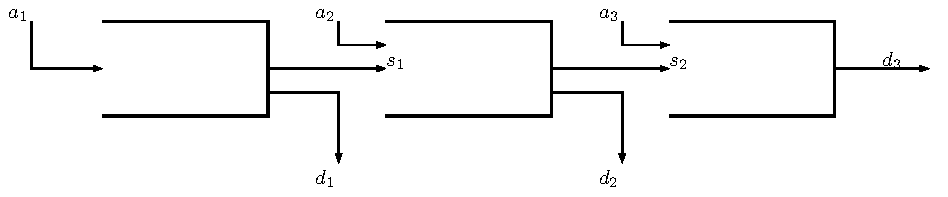
\includegraphics[scale=0.75]{figures/tandem.pdf}
 \caption{A system with 3 queues}
\end{figure}

\todo{ Precise description of the random process avec un dessin}

Our experimentations are made with the following set-up.
The central program is running on a MacBook Air, with a processor $2.2$ GHz Intel Core i$7$, and $8$ Go of RAM DDR$3$ at $1600$ MHz. The operating system of the machine is macOS High Sierra v$10.13.1$. The source code is compiled with  gcc version $7.1.0$ (Homebrew GCC $7.1.0$ --without-multilib).

Then the simulations of intervals are dispatched on up to $7$ Raspberry Pi 3 , Model B, with $1GB$ of RAM. Their operating system is  Raspbian GNU/Linux $8.0$, installed on a micro SD card element$14$ with a size of $8$GB. The source code is compiled with gcc version $4.9.2$ (Raspbian $4.9.2-10$).

All the machines are connected to a local network through an HP $14$-$10$ $8$G switch.

\todo{Description of the experimental settings: quel système d'exploitation/matériel/compilateur/librairies}

\todo{Experiments avec des jolies courbes et des interprétations}


Practical problems: cost of the network transmission, especially for transmitting long sequences.
-> measure the time of a two way trip for a small message and the time of sending an interval.
To say that in practice we will not compute the whole sequence but statistic on it which could help
reduce the use of the network.



\end{document}
